\documentclass[11pt,a4paper]{article}
% ══════════════════════════════════════════════════════════════════════════════
% Edexcel Further Mathematics (Core Pure 1) --- Shared LaTeX Preamble
% Elegant, Minimalist & Aesthetic Academic Design System
% ══════════════════════════════════════════════════════════════════════════════

\usepackage[a4paper, top=22mm, bottom=22mm, left=20mm, right=20mm]{geometry}
\usepackage{amsmath, amssymb, amsthm}
\usepackage{enumitem}
\usepackage{booktabs}
\usepackage{array}
\usepackage{parskip}
\usepackage{microtype}
\usepackage{fancyhdr}
\usepackage{titlesec}
\usepackage{mdframed}
\usepackage{xcolor}
\usepackage[hidelinks]{hyperref}
\usepackage{graphicx}
\usepackage{tikz}
\usepackage{pgfplots}
\pgfplotsset{compat=1.18}

% ── Refined Palette ───────────────────────────────────────────────────────────
\definecolor{primary}{gray}{0.10}
\definecolor{darkgray}{gray}{0.20}
\definecolor{medgray}{gray}{0.50}
\definecolor{lightgray}{gray}{0.96}
\definecolor{boxgray}{gray}{0.85}
\definecolor{accentline}{gray}{0.75}

% ── Section formatting ──────────────────────────────────────────────────────────
\titleformat{\section}[block]
  {\normalfont\bfseries\color{primary}}{}
  {0pt}{}[\vspace{1pt}{\color{accentline}\rule{\textwidth}{0.4pt}}\vspace{4pt}]
\titlespacing*{\section}{0pt}{14pt}{6pt}

% ── List formatting ─────────────────────────────────────────────────────────────
\setlist[enumerate,1]{label=\textbf{\arabic*.}, leftmargin=1.8em, itemsep=14pt}
\setlist[enumerate,2]{label=\textbf{(\alph*)}, leftmargin=1.8em, itemsep=6pt}

% ── Header / footer (Overlaps permanently eliminated) ─────────────────────────
\pagestyle{fancy}
\newcommand{\CPHeader}[2]{%
  \fancyhf{}%
  \setlength{\headheight}{22pt}%
  \renewcommand{\headrulewidth}{0.3pt}%
  \renewcommand{\headrule}{\hbox to\headwidth{\color{accentline}\leaders\hrule height \headrulewidth\hfill}}%
  \fancyhead[L]{\footnotesize\scshape\color{medgray} Core Pure 1: #1}%
  \fancyhead[R]{\footnotesize\color{medgray} Chapter \##2}%
  \renewcommand{\footrulewidth}{0.3pt}%
  \renewcommand{\footrule}{\hbox to\headwidth{\color{accentline}\leaders\hrule height \footrulewidth\hfill}}%
  \fancyfoot[L]{\footnotesize\color{medgray} Pearson Edexcel A-Level Further Mathematics $\cdot$ Core Pure 1}%
  \fancyfoot[C]{}% No center text to ensure zero collision with long titles
  \fancyfoot[R]{\footnotesize\color{medgray} \textbf{Henry.K} \enspace$\vert$\enspace Page \thepage}%
}

% ── Elegant Aesthetic Title Block ──────────────────────────────────────────────
\newcommand{\CPTitleBlock}[2]{%
  \vspace*{-8pt}
  \begin{center}
    {\footnotesize\scshape\color{medgray} Pearson Edexcel A-Level Further Mathematics \enspace$\cdot$\enspace Core Pure 1}\\[4pt]
    {\LARGE\bfseries\color{primary} #1}\\[4pt]
    {\small\color{darkgray} #2}\\[6pt]
    {\footnotesize\color{medgray} Problem Series authored by \textbf{Henry.K} \quad$\cdot$\quad 10 Exam Archetypes \quad$\cdot$\quad 65 Total Marks}\\[8pt]
    {\color{accentline}\rule{\textwidth}{0.5pt}}
  \end{center}
  \vspace{-6pt}
  \noindent{\footnotesize\itshape \textbf{Instructions:} Answer all ten questions. Full algebraic working must be shown for method marks; unsupported answers from calculators will not gain full credit. Give exact values in surd or fractional form unless specified otherwise.}\par
  \vspace{3pt}
  {\color{accentline}\rule{\textwidth}{0.5pt}}
  \vspace{8pt}
}

% ── Answer / Method / Investigate-further boxes ────────────────────────────────
\newmdenv[
  backgroundcolor=lightgray,
  linecolor=boxgray,
  linewidth=0.5pt,
  roundcorner=3pt,
  leftmargin=0pt, rightmargin=0pt,
  innerleftmargin=10pt, innerrightmargin=10pt,
  innertopmargin=6pt, innerbottommargin=6pt,
  skipabove=5pt, skipbelow=5pt
]{ansbox}

\newmdenv[
  backgroundcolor=lightgray!40,
  linecolor=darkgray,
  linewidth=1.2pt,
  leftline=true, rightline=false, topline=false, bottomline=false,
  leftmargin=0pt, rightmargin=0pt,
  innerleftmargin=10pt, innerrightmargin=8pt,
  innertopmargin=5pt, innerbottommargin=5pt,
  skipabove=5pt, skipbelow=7pt
]{invbox}

\newcommand{\ans}[1]{%
  \begin{ansbox}
    \textbf{Answer:} #1
  \end{ansbox}}

\newcommand{\method}[1]{%
  {\small\textbf{Method Criteria:}\par\vspace{2pt}#1}\par}

\newcommand{\inv}[1]{%
  \begin{invbox}
    \textbf{\small Deep Investigation:} {\small #1}
  \end{invbox}}

\newcommand{\qn}[1]{\textbf{#1.}\;}

\CPHeader{Volumes of Revolution}{5}

\begin{document}
\thispagestyle{plain}

\CPTitleBlock{Volumes of Revolution}{Problem Sheet 5 \enspace$\cdot$\enspace Rotations About Coordinate Axes, Parametric Solids \& Modelling}

\section*{Section A \quad Procedural \& Direct Foundations \hfill{\normalfont\footnotesize(Questions 1--3)}}
\begin{enumerate}

%── Q1 [DIR] ─────────────────────────────────────────────────────────────
\item \textbf{[DIR]} The region $R$ is bounded by the curve $y = 2\sqrt{x}$, the line $x = 1$, the line $x = 4$, and the $x$-axis.
\begin{center}
\begin{tikzpicture}[scale=0.9]
  \begin{axis}[
    axis lines=middle,
    xlabel={$x$}, ylabel={$y$},
    xmin=0, xmax=5, ymin=0, ymax=5,
    xtick={1, 4}, ytick={2, 4},
    domain=0:4.5, samples=100,
    width=7.5cm, height=5cm,
    axis line style={->, >=stealth, color=darkgray},
    tick label style={font=\footnotesize}
  ]
    \addplot[thick, color=primary] {2*sqrt(x)} node[right, font=\small] {$y = 2\sqrt{x}$};
    \addplot[fill=lightgray, draw=accentline, domain=1:4] {2*sqrt(x)} \closedcycle;
    \draw[dashed, color=medgray] (axis cs:1,0) -- (axis cs:1,2);
    \draw[dashed, color=medgray] (axis cs:4,0) -- (axis cs:4,4);
    \node at (axis cs:2.5, 1.2) [font=\small] {$R$};
  \end{axis}
  \draw[->, >=stealth, color=darkgray, thick] (7.2, 0.4) arc (-80:240:0.35 and 0.6);
  \node at (7.8, 0.8) [font=\footnotesize\color{medgray}] {$2\pi$};
\end{tikzpicture}
\end{center}
The region $R$ is rotated through $2\pi$ radians about the $x$-axis to form a solid of revolution. Find the exact volume of the solid generated, giving your answer in terms of $\pi$. \hfill{\textbf{[4 marks]}}

%── Q2 [DIR] ─────────────────────────────────────────────────────────────
\item \textbf{[DIR]} The curve $C$ has equation $y = x^3$, $x \ge 0$.
The region bounded by $C$, the $y$-axis, and the horizontal lines $y = 1$ and $y = 8$ is rotated through $2\pi$ radians about the $y$-axis.
\begin{enumerate}[label=(\alph*)]
  \item Express $x^2$ in terms of $y$. \hfill{\textbf{[1 mark]}}
  \item Find the exact volume of the solid formed, giving your answer as a multiple of $\pi$. \hfill{\textbf{[3 marks]}}
\end{enumerate}

%── Q3 [DIR] ─────────────────────────────────────────────────────────────
\item \textbf{[DIR]} A curve is defined parametrically by
\[
x = 3\cos\theta, \quad y = 2\sin\theta, \quad 0 \le \theta \le \frac{\pi}{2}
\]
The region bounded by this curve, the positive $x$-axis, and the positive $y$-axis is rotated through $2\pi$ radians about the $x$-axis.
\begin{enumerate}[label=(\alph*)]
  \item Show that the volume $V$ of the solid of revolution is given by
  \[
  V = 12\pi \int_0^{\pi/2} \sin^3\theta \, d\theta
  \]
  \hfill{\textbf{[3 marks]}}
  \item Using the identity $\sin^3\theta = \sin\theta(1 - \cos^2\theta)$, evaluate $V$ exactly. \hfill{\textbf{[3 marks]}}
\end{enumerate}

\end{enumerate}

\section*{Section B \quad Reverse Parameters \& Analysis \hfill{\normalfont\footnotesize(Questions 4--6)}}
\begin{enumerate}[resume]

%── Q4 [REV] ─────────────────────────────────────────────────────────────
\item \textbf{[REV]} A curve has parametric equations
\[
x = 2t^2, \quad y = t^3, \quad 0 \le t \le 2
\]
The finite region bounded by the curve, the line $y = 8$, and the $y$-axis is rotated through $2\pi$ radians about the $y$-axis.
Find the exact volume of the solid generated, giving your answer in the form $\dfrac{a\pi}{b}$, where $a$ and $b$ are coprime integers. \hfill{\textbf{[5 marks]}}

%── Q5 [REV] ─────────────────────────────────────────────────────────────
\item \textbf{[REV]} The finite region $R$ is enclosed between the line $y = x$ and the parabola $y = x^2$.
\begin{center}
\begin{tikzpicture}[scale=0.9]
  \begin{axis}[
    axis lines=middle,
    xlabel={$x$}, ylabel={$y$},
    xmin=0, xmax=1.4, ymin=0, ymax=1.4,
    xtick={1}, ytick={1},
    domain=0:1.2, samples=80,
    width=6.5cm, height=5cm,
    axis line style={->, >=stealth, color=darkgray},
    tick label style={font=\footnotesize}
  ]
    \addplot[thick, color=darkgray] {x} node[pos=0.9, above left, font=\footnotesize] {$y = x$};
    \addplot[thick, color=primary] {x^2} node[pos=0.9, below right, font=\footnotesize] {$y = x^2$};
    \addplot[fill=lightgray, domain=0:1] {x} \closedcycle;
    \addplot[fill=white, domain=0:1] {x^2} \closedcycle;
    \draw[dashed, color=medgray] (axis cs:1,0) -- (axis cs:1,1) -- (axis cs:0,1);
    \node at (axis cs:0.55, 0.4) [font=\small] {$R$};
  \end{axis}
  \draw[->, >=stealth, color=darkgray, thick] (6.2, 0.3) arc (-80:240:0.35 and 0.55);
  \node at (6.8, 0.7) [font=\footnotesize\color{medgray}] {$2\pi$};
\end{tikzpicture}
\end{center}
The region $R$ is rotated through $360^\circ$ about the $x$-axis to create a hollow solid of revolution.
Find the exact volume of the solid generated. \hfill{\textbf{[5 marks]}}

%── Q6 [REV] ─────────────────────────────────────────────────────────────
\item \textbf{[REV]} The region enclosed by the parabola $y = 4 - x^2$ and the coordinate axes in the first quadrant is rotated through $2\pi$ radians about the $y$-axis.
\begin{enumerate}[label=(\alph*)]
  \item Write down the integral with respect to $y$ that represents this volume. \hfill{\textbf{[2 marks]}}
  \item Hence find the exact volume of the resulting paraboloid. \hfill{\textbf{[3 marks]}}
\end{enumerate}

\end{enumerate}

\section*{Section C \quad Proof, Geometry \& Multi-step \hfill{\normalfont\footnotesize(Questions 7--10)}}
\begin{enumerate}[resume]

%── Q7 [CTX] ─────────────────────────────────────────────────────────────
\item \textbf{[CTX]} A glass bowl is designed by rotating the curve $x = 2\sqrt{y}$ for $0 \le y \le 4$ through $2\pi$ radians about the $y$-axis, where $x$ and $y$ are measured in centimetres.
\begin{center}
\begin{tikzpicture}[scale=0.85]
  \begin{axis}[
    axis lines=middle,
    xlabel={$x$ (cm)}, ylabel={$y$ (cm)},
    xmin=-5.5, xmax=5.5, ymin=0, ymax=5,
    xtick={-4, 4}, ytick={4},
    domain=0:4, samples=60,
    width=8cm, height=5.5cm,
    axis line style={->, >=stealth, color=darkgray},
    tick label style={font=\footnotesize}
  ]
    \addplot[thick, color=primary] ({2*sqrt(x)}, {x});
    \addplot[thick, color=primary] ({-2*sqrt(x)}, {x});
    \addplot[fill=lightgray!60, opacity=0.8] ({2*sqrt(x)}, {x}) -- (-4,4) -- cycle;
    \draw[dashed, color=medgray] (axis cs:-4,4) -- (axis cs:4,4);
    \node at (axis cs:0, 2) [font=\small] {Bowl Interior};
  \end{axis}
\end{tikzpicture}
\end{center}
\begin{enumerate}[label=(\alph*)]
  \item Show that the total internal capacity of the bowl is $32\pi \text{ cm}^3$. \hfill{\textbf{[3 marks]}}
  \item Water is poured into the bowl at a constant rate of $6\pi \text{ cm}^3/\text{s}$. Find the rate at which the water level is rising, $\dfrac{dh}{dt}$, when the depth $h = 3 \text{ cm}$. \hfill{\textbf{[4 marks]}}
\end{enumerate}

%── Q8 [REV] ─────────────────────────────────────────────────────────────
\item \textbf{[REV]} The curve $C$ has equation $y = \dfrac{k}{x}$ for $1 \le x \le 4$, where $k$ is a positive constant.
The region bounded by $C$, the $x$-axis, and the lines $x = 1$ and $x = 4$ is rotated through $2\pi$ radians about the $x$-axis.
Given that the volume of the resulting solid is $12\pi$, find the exact integer value of $k$. \hfill{\textbf{[5 marks]}}

%── Q9 [SYN] ─────────────────────────────────────────────────────────────
\item \textbf{[SYN]} 
\begin{enumerate}[label=(\alph*)]
  \item The region bounded by the curve $y = \sqrt{\cos x}$, the coordinate axes, and the vertical line $x = \dfrac{\pi}{2}$ is rotated through $2\pi$ radians about the $x$-axis. Find the exact volume of the solid generated. \hfill{\textbf{[3 marks]}}
  \item Verify that the answer obtained in (a) is strictly less than the volume of a cylinder of radius 1 and height $\dfrac{\pi}{2}$. \hfill{\textbf{[2 marks]}}
\end{enumerate}

%── Q10 [SYN] ────────────────────────────────────────────────────────────
\item \textbf{[SYN]} The straight line $y = 2 + \dfrac{1}{2}x$ for $0 \le x \le 4$ is rotated through $2\pi$ radians about the $x$-axis to form a frustum of a cone.
\begin{enumerate}[label=(\alph*)]
  \item Use calculus to prove that the volume of the frustum is $\dfrac{112\pi}{3}$. \hfill{\textbf{[4 marks]}}
  \item The geometric formula for the volume of a frustum of height $h$ with end radii $r_1$ and $r_2$ is
  \[
  V_{\text{geom}} = \frac{1}{3}\pi h(r_1^2 + r_1 r_2 + r_2^2)
  \]
  Verify that this formula yields the identical result. \hfill{\textbf{[3 marks]}}
\end{enumerate}

\end{enumerate}

\vspace{14pt}
\begin{center}
  {\color{accentline}\rule{0.4\textwidth}{0.4pt}}\\[5pt]
  {\footnotesize\itshape\color{medgray} ``Nature does not hurry, yet everything is accomplished.''}\\[2pt]
  {\scriptsize\scshape\color{medgray} Lao Tzu}\\[5pt]
  {\color{accentline}\rule{0.4\textwidth}{0.4pt}}
\end{center}

\end{document}
